\chapter[Diagramas]{Diagramas}
Durante o desenvolvimento do projeto, alguns diagramas foram elaborados para sincronização de pensamento da equipe e entendimento coletivo.

Como forma organização, separamos os diagramas em dois grupos, representados pelas seções a seguir.

 \section{Banco de Dados}
  Dentre os diagramas construídos, dois consistem no banco de dados, para entendimento da conexão entre as entidades do sistema, sendo um deles Diagrama de Entidade-Relacionamento, que consiste na \autoref{fig:der} e mostra o relacionamento entre as entidades do sistema, enquanto o outro consiste no Diagrama do Modelo Lógico do banco de dados da aplicação, representado na \autoref{fig:bdml}, mostrando essas relacionamentos de forma menos abstrata, já com os campos de cada tabela e seus tipos.

  \begin{figure}[!htb]
        \centering
        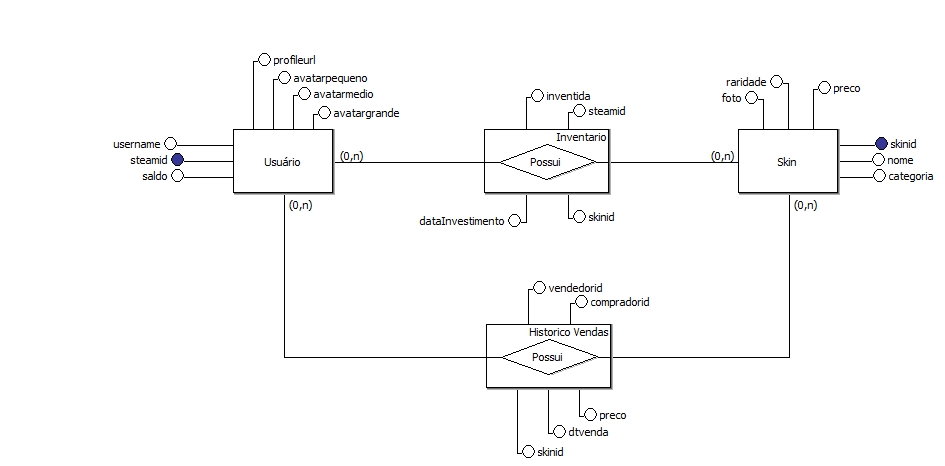
\includegraphics[scale=0.5]{Imagens/Relacionamento.png}
        \caption{Banco de Dados - Diagrama Entidade Relacionamento}
        \label{fig:der}
 \end{figure}

\begin{figure}[!htb]
	\centering
	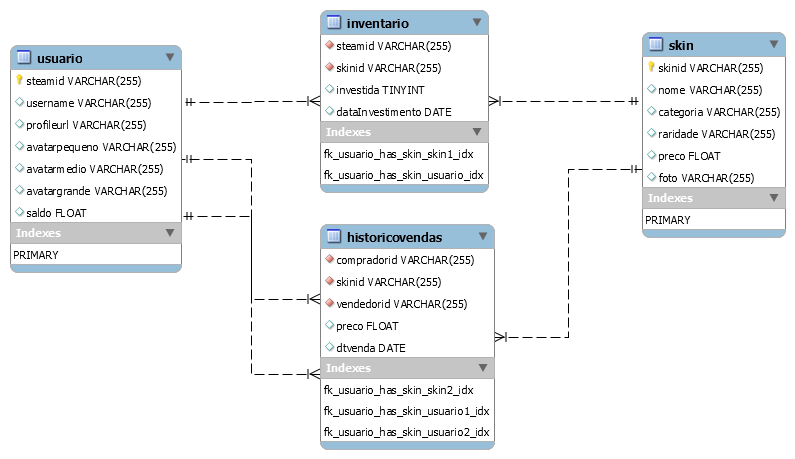
\includegraphics[scale=0.6]{Imagens/Logico.png}
	\caption{Banco de Dados - Modelo Lógico}
	\label{fig:bdml}
\end{figure}
\clearpage

\section{Diagramas de Atividade}
Além desses dois diagramas apresentados acima, três Diagramas de Atividade foram construídos para auxiliar no alinhamento de ideias do grupo e entendimento das funcionalidades. 

O diagrama representado na \autoref{fig:dami} consiste no funcionamento do mecanismo de inventário do projeto, enquanto a \autoref{fig:damdt} representa o funcionamento da mecânica de Day Trade e a \autoref{fig:damc} representa o sistema de carteira da aplicação.

	\begin{figure}[!htb]
		\centering
		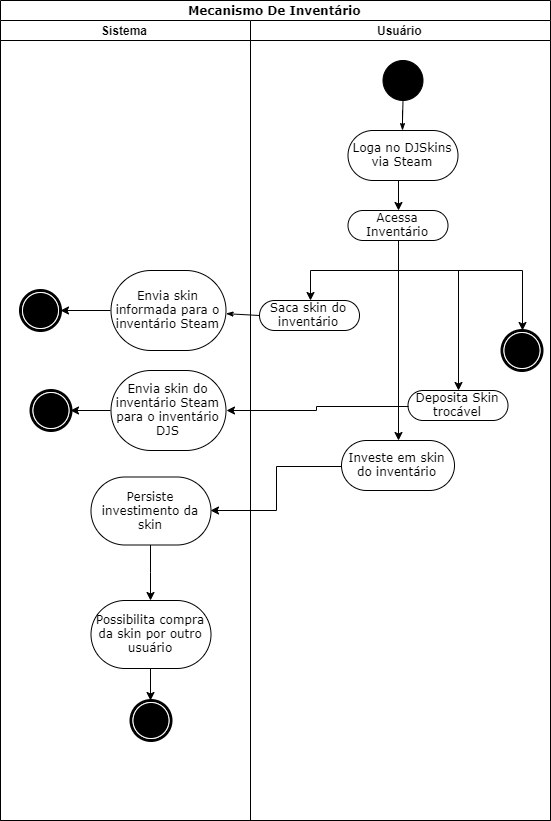
\includegraphics[scale=0.6]{Imagens/mec-inventario.png}
		\caption{Diagrama de Atividades - Mecanismo de Inventário}
		\label{fig:dami}
	\end{figure}
	
	\begin{figure}[!htb]
		\centering
		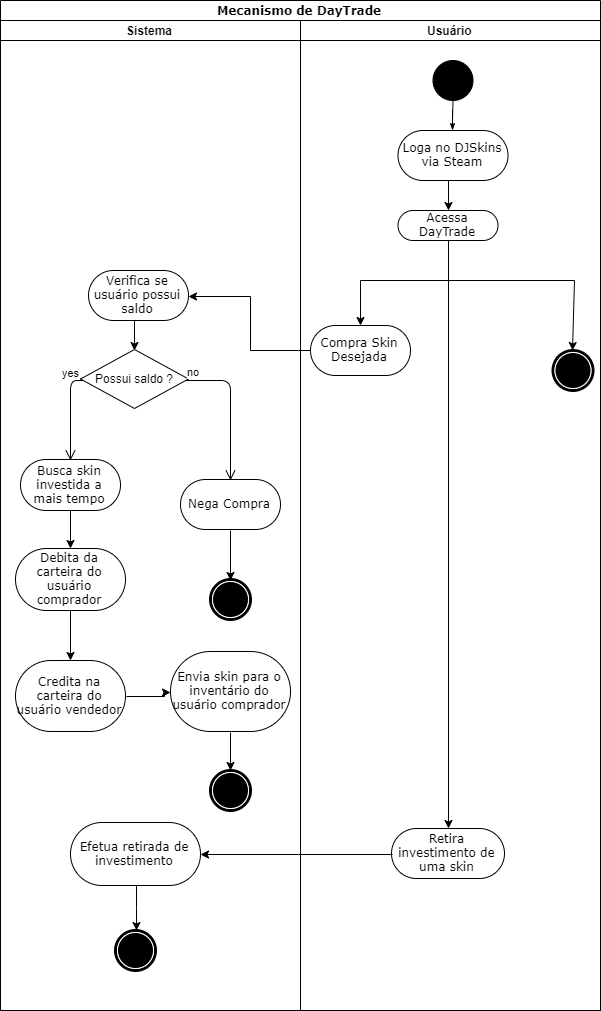
\includegraphics[scale=0.6]{Imagens/mec-daytrade.png}
		\caption{Diagrama de Atividades - Mecanismo de Day Trade}
		\label{fig:damdt}
	\end{figure}
	
	\begin{figure}[!htb]
		\centering
		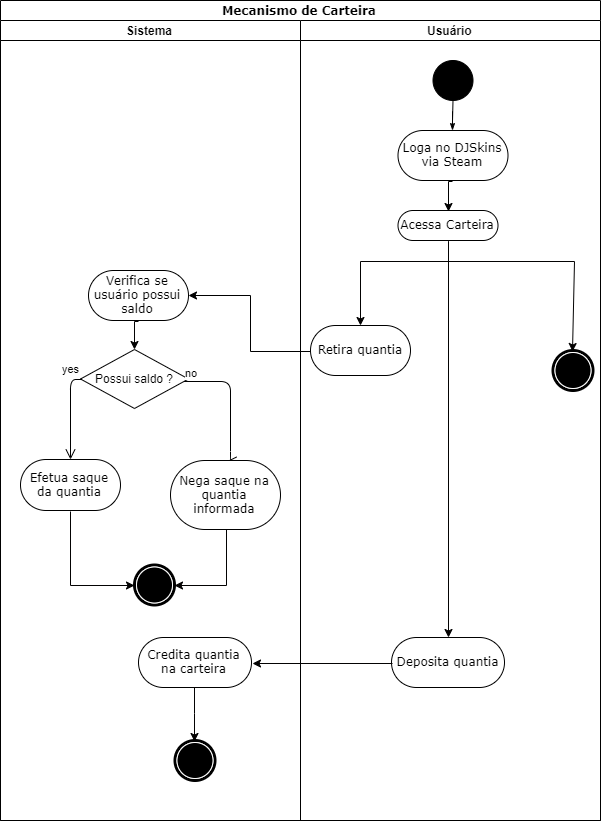
\includegraphics[scale=0.6]{Imagens/mec-carteira.png}
		\caption{Diagrama de Atividades - Mecanismo de Carteira}
		\label{fig:damc}
	\end{figure}